% !TEX TS-program = pdflatex
% !TEX encoding = UTF-8 Unicode

% This is a simple template for a LaTeX document using the "article" class.
% See "book", "report", "letter" for other types of document.

\documentclass[11pt]{article} % use larger type; default would be 10pt
\usepackage[T2A]{fontenc}
\usepackage[serbianc]{babel}
\usepackage[utf8]{inputenc} % set input encoding (not needed with XeLaTeX)
\usepackage{lipsum}
\usepackage{setspace}
\usepackage{listings}
\usepackage{xcolor}
\usepackage{graphicx}
\graphicspath{{./img/}}

%Za reference
\usepackage[style=verbose]{biblatex}

\usepackage{biblatex}
\addbibresource{cite.bib}

%za pajton
\definecolor{codegreen}{rgb}{0,0.6,0}
\definecolor{codegray}{rgb}{0.5,0.5,0.5}
\definecolor{codepurple}{rgb}{0.58,0,0.82}
\definecolor{backcolour}{rgb}{0.95,0.95,0.92}

\lstdefinestyle{mystyle}{
    backgroundcolor=\color{backcolour},   
    commentstyle=\color{codegreen},
    keywordstyle=\color{magenta},
    numberstyle=\tiny\color{codegray},
    stringstyle=\color{codepurple},
    basicstyle=\ttfamily\footnotesize,
    breakatwhitespace=false,         
    breaklines=true,                 
    captionpos=b,                    
    keepspaces=true,                 
    numbers=left,                    
    numbersep=5pt,                  
    showspaces=false,                
    showstringspaces=false,
    showtabs=false,                  
    tabsize=2
}
\lstset{style=mystyle}

\title{Домаћи задатак I \\  Системи за подршку одлучивању}
\author{Матеја Вујсић 405/2022}

%%% Examples of Article customizations
% These packages are optional, depending whether you want the features they provide.
% See the LaTeX Companion or other references for full information.

%%% PAGE DIMENSIONS
\usepackage{geometry} % to change the page dimensions
\geometry{a4paper} % or letterpaper (US) or a5paper or....
% \geometry{margin=2in} % for example, change the margins to 2 inches all round
% \geometry{landscape} % set up the page for landscape
%   read geometry.pdf for detailed page layout information
% support the \includegraphics command and options

% \usepackage[parfill]{parskip} % Activate to begin paragraphs with an empty line rather than an indent

%%% PACKAGES
\usepackage{booktabs} % for much better looking tables
\usepackage{array} % for better arrays (eg matrices) in maths
\usepackage{paralist} % very flexible & customisable lists (eg. enumerate/itemize, etc.)
\usepackage{verbatim} % adds environment for commenting out blocks of text & for better verbatim
\usepackage{subfig} % make it possible to include more than one captioned figure/table in a single float
% These packages are all incorporated in the memoir class to one degree or another...

%%% HEADERS & FOOTERS % header line width
\usepackage{fancyhdr} % This should be set AFTER setting up the page geometry
\pagestyle{fancy}
\renewcommand{\headrulewidth}{0pt} % customise the layout...
\lhead{Факултет инжењерских наука}\chead{}\rhead{Системи за подршку одлучивању}
\lfoot{}\cfoot{\thepage}\rfoot{}

\renewcommand{\sectionmark}[1]{ \markright{#1}{} }
\renewcommand{\headrulewidth}{0.4pt}

%%% SECTION TITLE APPEARANCE
\usepackage{sectsty}
\allsectionsfont{\sffamily\mdseries\upshape\textbf} % (See the fntguide.pdf for font help)
% (This matches ConTeXt defaults)

%%% ToC (table of contents) APPEARANCE

\usepackage[nottoc,notlof,notlot]{tocbibind} % Put the bibliography in the ToC
\usepackage[titles,subfigure]{tocloft} % Alter the style of the Table of Contents
\renewcommand{\cftsecfont}{\rmfamily\mdseries\upshape\normalfont\bfseries}
\renewcommand{\cftsecpagefont}{\rmfamily\mdseries\upshape} % No bold!

\usepackage{hyperref}
\hypersetup{linktoc=page}

%%% END Article customizations

%%% The "real" document content comes below...


%\date{} % Activate to display a given date or no date (if empty),
         % otherwise the current date is printed 

\begin{document}
\makeatletter
    \begin{titlepage}
        \begin{center}
            
\includegraphics[width=0.2\linewidth]{grb-faks.png}\\[7ex]
            {\huge \bfseries  \@title }\\[2ex] 
            {\LARGE  \@author}\\[50ex] 
            {\large \@date}
        \end{center}
    \end{titlepage}
\makeatother
\thispagestyle{empty}
\newpage
\newpage

\doublespacing
\tableofcontents
\singlespacing

\newpage
\section{Увод}
Класификација је проблем када одреженој појави желимо да дамо одређену класу. На пример, времеска прогноза може класификовати дан као кишни или не кишни. Алгоритми који улазни скуп података мапирају на у одређену класу називају се класификатори односно класификациони алгоритми. Постоји неколико различитих врста класификатора од који свака има одређене предности и мане. У односу на скуп улазних података, тачније њихове величине и типа, треба користити различите типове класификатора. \\
\linebreak
У овом домаћем задатку биће речи о следећим класификаторима:
\begin{itemize}
	\item Logistic Regression
	\item Decision Tree
	\item Random Forest
	\item Naïve Bayes Classifier
	\item Support Vector Machine (SVM)
	\item K Nearest Neighbors (KNN)
\end{itemize}

Поред описа алгоритама, биће приказани критеријуми и парамтери које је могуће оптимизовати и библиотеке потребне за њихово тренирање у програмском језику Python.  
\newpage

\section{Logistic Regression}

Логичка регресија(енгл. Logistic regression) је најчешће коришћен класификациони алгоритам. То је тип логичке регресије у којој је зависна варијабла искључиво дихотома тј. може попримити бинарне вредности 0 или 1, или између њих. Овај алгоритам улазном скупу додељује вредност између 0 и 1 која означава вероватноћу
припадности одређеној категорији на излазу. Затим се додељена вредност упоређује са
одређеним степеном активације (threshold вредност), да би се одредила припадност класи.

Додељене вредности се представљају на логистичкој кривој (сигмоидној функцији)
као што је приказано на слици 1.

\begin{figure}[h]
	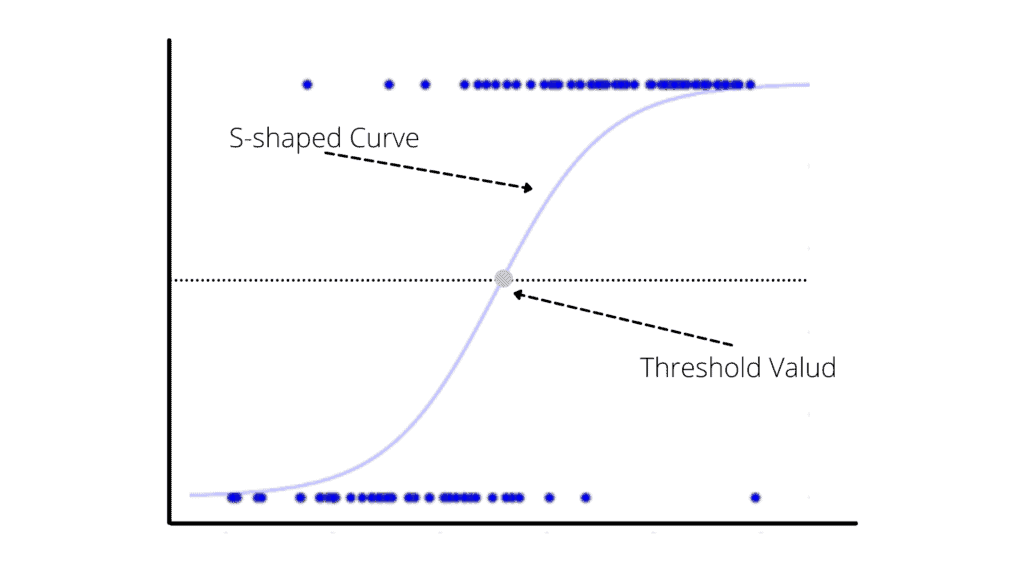
\includegraphics[scale=0.4]{Logistic-regression-using-python-s-shpaed}
	\caption{Логистичка регресија}
\end{figure}

Мана је што лако долази до преобучавања када је количина података заобучавање мала и неопходна је регуларизација. Такође може се рећи да овај алгоритам ради са вишекласним излазима, али у тим случајевима прецизност није загарантована.

Логистичка регресија може бити биномијална, мултиномијална и ординална, при
чему тип зависи од броја класа и њиховог односа.

\subsection{Python имплементација}
За прављење модела класификатора логичке регресије у пајтону користи се библиотека \textbf{scikit-learn}. Само креирање модела је тривијалано (једна линија кода).
\begin{lstlisting}[language=Python,title=Пример 1. Логичка регресија]
# Import sckikit-learn statment
from sklearn.linear_model import LogisticRegression
model = LogisticRegression(solver='liblinear', random_state=0)
\end{lstlisting}

Постоји 15 опционих параметара при креирању који су задужени за понашање и приступ модела који се тренира. \\
Највешћемо само неке најважније:

\begin{itemize}
	\item \textbf{solver} - дефинише солвер који ће се користити за обучавања модела.
	\item \textbf{max\_iter} - дефинише максимални број итерација солвера који ће се користити приликом обучавања.
	\item \textbf{class\_weight} - дефинше тежину класа, опционо свака класа је исте тежине.
	\item \textbf{random\_state} - дефинше и генерише псеудослучајни број који се касније користи.
\end{itemize}
\section{Decision Tree}
Стабло одлуке(енг. Decision Tree) је један од алгоритама за решавања проблема класификације. Алгоритам се своди на формирање стабла одлучивања на основу тумачења улазног скупа података. Стабла се састоје из корена, чворова и листова. (Слика 2.) Корен(бело) је почетни чвор(бело), а листови(зелено и црвено) представљају чворове одлуке, тј. представљају крајње чворове у стаблу одлучивања. У тренутку када алгоритам наиђе на лист, одлука је донета и процес класификације је завршен.
\\
\begin{figure}[h]
\centering
	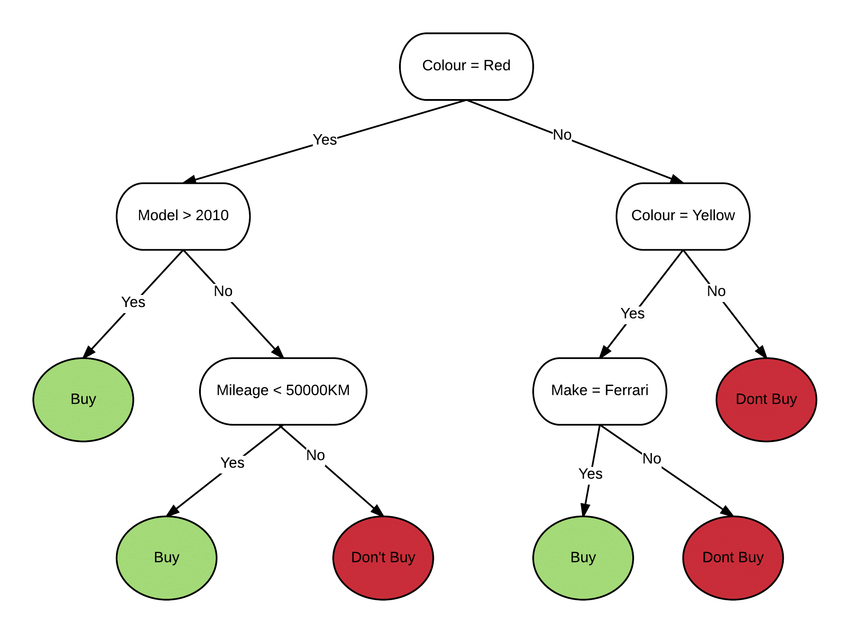
\includegraphics[scale=0.3]{decision_tree}
	\caption{Графички приказ стабло одлуке примеру улазних података}
\end{figure}

Као једна од предности овог алгоритма истиче се то да за мали скуп конкретних улазних података је могуће формирати стабло одлуке. Такође је и могуће лако графички приказати ток одлуке(Слика 2.).

Стабла одлуке су стабилна уколико су разлике између података уочљиве и конкретне. У супротном постају нестабилна и самим тим смањује се тачност одлуке. Нестабилна стабла захтевају потпуну измену структуре, додавањем минималних измена у сету података.
\subsection{Python имплементација}

За прављење модела класификатора стабла одлуке у пајтон програмском језику користи се библиотека \textbf{scikit-learn}. Само креирање модела је тривијалано (једна линија кода).

\begin{lstlisting}[language=Python,title=Пример 2. Стабло одлуке]
 # Decision Tree 
 from sklearn.tree import DecisionTreeClassifier  
 classifier = DecisionTreeClassifier(criterion='entropy', random_state=0)   
\end{lstlisting}

Најважнији параметри класе DecisionTreeClassifier су:
\begin{itemize}
	\item \textbf{max\_depth} - дефинише максималну дубину стабла.
	\item \textbf{max\_leaf\_nodes} - дефинише максималан број излазних листа методом best-first.
	\item \textbf{class\_weight} - дефинше тежину класа, опционо свака класа је исте тежине.
\end{itemize}

\section{Random Forest}

\begin{figure}[h]
\centering
	\includegraphics[scale=0.5]{random_forest}
	\caption{Графички приказ - random forest} 
\end{figure}

Назив шума потиче од чињенице да се овај алгоритам састоји од више стабала
одлуке(Слика 3.\footnote{Слика преузета са https://www.freecodecamp.org/news/how-to-use-the-tree-based-algorithm-for-machine-learning/ датума 16.10.2022. у 11 часова.}.).

Резултат таквог једног стабла које је тренирано на један начин и с једним
скупом података најчешће неће бити најпрецизнији ако стабло има малу дубину, а
уколико има велику дубину може доћи до ткз.претренираности(енг. overfiting).

Због наведених проблема јавила се идеја случајних шума. Алгоритам случајних
шума је такав да постоји више стабала одлуке који уче насумично из одабраног скупа
података, одакле и потиче назив случајних шума, да би тиме стабла била што
разноврснија. 

Такође, због велике дубине стабла, решава се и проблем недовољно добре
интерпретације веза између варијабли унутар употребљеног скупа података(енг.
underfiting). Решавање проблема underfiting-а и overfiting-а представља главну предност
алгоритма случајних шума.

\subsection{Python имплементација}

За прављење модела класификатора случајних шума у пајтон програмском језику користи се библиотека \textbf{scikit-learn}. Само креирање модела је тривијалано (једна линија кода).

\begin{lstlisting}[language=Python,title=Пример 3. Класификатор случајних шума]
#Import Random Forest Model
from sklearn.ensemble import RandomForestClassifier

#Create a Gaussian Classifier
clf = RandomForestClassifier(n_estimators=100)
\end{lstlisting}
\begin{itemize}
	\item \textbf{n\_estimators} - дефинише број стабала одлуке.
	\item \textbf{max\_depth} - дефинише максималну дубину стабла.
	\item \textbf{class\_weight} - дефинше тежину класа, опционо свака класа је исте тежине.
\end{itemize}

\section{Naïve Bayes Classifier}

Наивни Бајесов класификатор ради на принципу Бајесове теореме. Алгоритам претпоставља независност међу подацима и израчунава вероватноћу припадања излаза свакој од могућих класа на основу припадности својих улаза свакој од могућих класа унутар скупа података. На самом крају алгоритам доноси одлуку да излаз припада класи са највећом вероватноћом.\footnote{Преведено са https://scikit-learn.org/stable/modules/naive_bayes.html1}

%Преведено са https://scikit-learn.org/stable/modules/naive_bayes.html

Постоји више врста наивног Бајесовог класификатора, од којих свака има своје почетне претпоставке које могу унапредити прецизност добијеног излаза.(1)

\begin{equation}
P(y|_{x1},.._{xn}) = \frac{P(y)P(x_{1},..x_{n}|y)}{P(y)P(x_{1},..x_{n})}
\end{equation}

Гаусов наивни Бајес(1) полази од претпоставке да улазни подаци потпадају под гаусову расподелу. Осим самог појављивања елемената у скупу података, у коначну одлуку улазе параметри ми и сигма који представљају позицију и ширину претпостављене гаусове криве(2).\footnote{Преузето са https://scikit-learn.org/stable/modules/naive_bayes.html }


\begin{equation}
P(x_{i}|y) = \frac{1}{\sqrt{2\Pi{}(\delta})^2}\exp{(-\frac{x_{i}-\eta_{y}^2}{2\delta^2_{y}})}
\end{equation}

Мултиномијални наивни Бајес(3) је најпопуларнији класификатор када је у питању класификација текстуалних података. Користи се у случајевима када постоји велики број могућих излатних класа, па се као решење добија вектор вероватноћа θу.
\begin{equation}
\theta_{yi} = \frac{N_{yi}+a}{N_{y}+\alpha n }
\end{equation}

Категорички наивни Бајес функционише на сличан начин мултиномијалном наивном Бајесу. Користи се над неизбалансираним сетовима података, односно сетовима у којима су неке класе знатно доминантније у поређењу са осталима. Овај алгоритам додељује тежинске коефицијенте класама како би се постигао бољи баланс (4).

\begin{equation}
\theta_{ci} = \frac{a_{i}+\sum_{j:y\neq c}d_{ij}}{a_{i}+\sum_{j:y\neq c}\sum{k}{d_{ij}}}
\end{equation}

\begin{equation}
w_{ci} = \log{\theta_{ci}}
\end{equation}

\begin{equation}
w_{ci} = \frac{w_{ci}}{\sum{j}{|w_{ci}|}}
\end{equation}

Бернулијев наивни Бајес се користи над подацим који потпадају под мултиваријантну Бернулијеву расподелу, односно када постоји широк спектар података, али је за сваки предпостављена бинарна вредност [4].

\begin{equation}
P(x_{i}|y) = P(i|y)x_{i} + (1 - P(i|y))(1-x_{i})
\end{equation}

Наивни Бајесов класификатор је најбржи класификатор од свих споменутих у овом раду. Међутим важи за класификатор са лошим способностима генерализације јер је лако довести га и у under-fitted као и у over-fitted стање. Поврх тога захтева велики скуп података за тренирање како би се избегле нула вероватноће.

\subsection{Python имплементација}

За прављење модела класификатора наивног бајаса у пајтон програмском језику користи се библиотека \textbf{scikit-learn}. Само креирање модела је тривијалано (једна линија кода).

\begin{lstlisting}[language=Python,title=Пример 4. Наивни Бајас]
from sklearn.naive_bayes import GaussianNB
gnb = GaussianNB()
\end{lstlisting}

Параметри:

\begin{itemize}
	\item \textbf{class\_count\_} - дефинише број тренинг узорака у свакој класи.
	\item \textbf{class\_prior} - дефинише вероватноћу сваке класе.
	\item \textbf{n\_features\_in} - дефинше broj параметара.
\end{itemize}

\section{Support Vector Machine}

Support Vector Machine је скуп метода за супервизорно обучавање, које се
користе за решавање проблема класификације и регресије.

Алгоритам функционише тако што прима n-димензиони скуп података и на
основу њега креира n-димензиони систем у оквиру кога су подаци представљени.
Поента је да алгоритам успе да креира n-димензионе хиперравни помоћу којих ће
систем поделити на делове а ти делови ће у ствари бити класе. За одјавање нпр две
класе тачака постоји много могућих хиперравни које се могу изабрати. Циљ је да се
пронађе раван која има максимално растојање између тачака података обе класе.

\begin{figure}[h]
\centering
	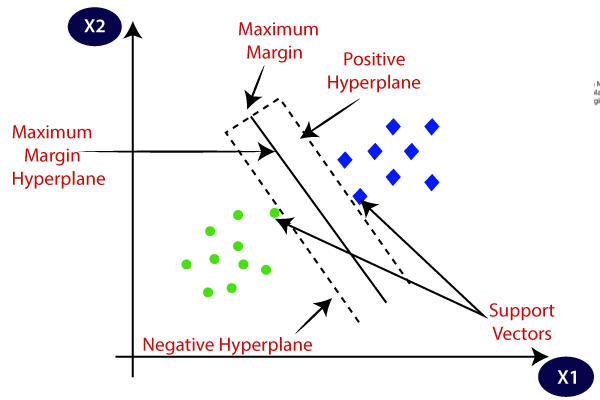
\includegraphics[scale=0.5]{support-vector-machine-algorithm}
	\caption{Support Vector Machine} 
\end{figure}

Предности класификатора су то што ради релативно добро када постоји јасна
граница раздвајања класа, ефикасан је у вишедимензионим просторима и у
случајевима када је број димензија већи од броја узорака.

Међутим овај алгоритам погодан је на изузетно малим скуповима података.
\subsection{Python имплементација}

За прављење модела класификатора потпорних вектора у пајтон програмском језику користи се библиотека \textbf{scikit-learn}. Само креирање модела је тривијалано (једна линија кода).

\begin{lstlisting}[language=Python,title=Пример 3. Класификатор Метода потпорних вектора]
#Import SVC
from sklearn.svm import LinearSVC

#Create a SVM instance
svm = SVM()
\end{lstlisting}
\begin{itemize}
	\item \textbf{degree} - дефинише степен полиномијане функције апроксимације.
	\item \textbf{class\_weight} - дефинше тежину класа, опционо свака класа је исте тежине.
\end{itemize}

\section{K Nearest Neighbour (KNN)}

\begin{figure}[h]
\centering
	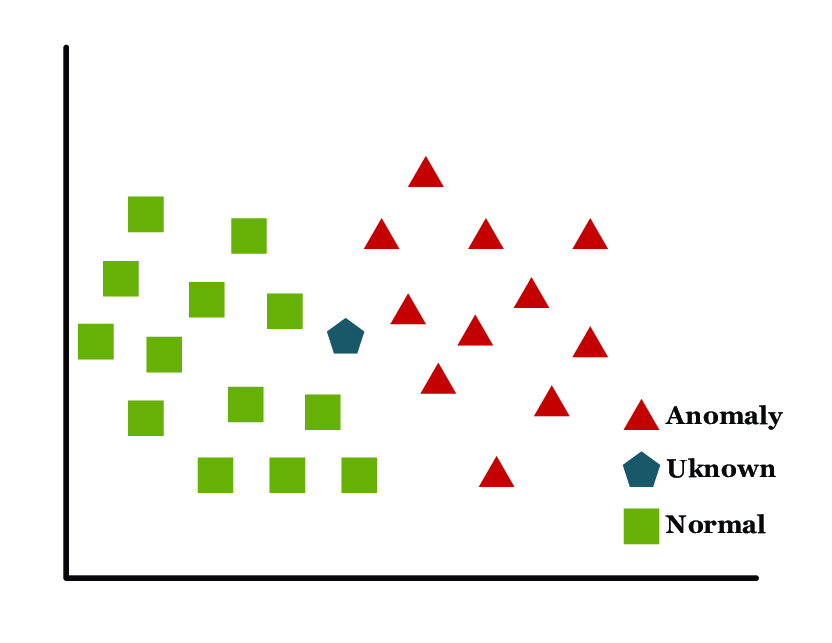
\includegraphics[scale=0.3]{K-Nearest-Neighbor-KNN-classification-principle}
	\caption{KNN алгоритам} 
\end{figure}

Последњи класификациони алгоритам који ће бити обрађен у овом раду је алгоритам К-најближих суседа(енг. K-Nearest Neighbor). 

Oвај алгоритам класификује тачку посматрања у односу на то како су суседи класификовани
, тачније, он посматра све примерке у скупу подата и класификује нове примерке на основу сличности. У овом алгоритму K представља параметар који означава број најближих суседа коју су укључени, тачније гледа суседе у околини и на основу њих класификује нови примерак. \footnote{Преузето са https://rti.etf.bg.ac.rs/rti/ms1psz/pdf/kNN.pdf}

Избор праве вредности за фактор K је процес који се назива ''подешавање параметара''. Циљ је обезбедити што већу прецизност модела а то значи одредити што бољи фактор параметара K.

Овај класификатор је најједноставнији за имплементацију, и ради добро са свим величинама скупова познатих података. Meђутим највећа мана овог алгоритма јесте велико време чекања при одређивању К најближих суседа, јер алгоритам мора израчунати раздаљину од сваке познате тачке система до новог члана. Ово утиче на време извршавања самог алгоритма. 

Постоји неколико алгоритама(једначина) за израчунавање растојања између тачака. Неке од ових су:

\begin{itemize}
	\item \textbf{Канабера растојање} 
	\item \textbf{Минковски растојање} 
	\item \textbf{Менхетн растојање}
	\item \textbf{Чебишевљево растојање}
	\item \textbf{Еуклидово растојање} 
\end{itemize}

\subsection{Python имплементација}

За прављење модела класификатора К-најближих суседа у пајтон програмском језику користи се библиотека \textbf{scikit-learn}. Само креирање модела је тривијалано (једна линија кода).

\begin{lstlisting}[language=Python,title=Пример 3. Класификатор KNN \footnote{n\_neighbors jе 4, што значи да ће се предикција будуће тачке темељити на 4 наближа суседа} ]
#Import KNN from sklearn.neighbors

from sklearn.neighbors import KNeighborsRegressor
knn_model = KNeighborsRegressor(n_neighbors = 4)

\end{lstlisting}

\begin{itemize}
	\item \textbf{n\_neighbors} - дефинише колико ће се суседа користити у класификовању будуће тачке.
\end{itemize}

\newpage
\section{Закључак}

Поред регресије, класификација је један од најчешћих проблема у областима машинског и дубоког учења. Примена самих алгоритама класификације највише зависи од добре анализе скупа података. Анализа неког скупа подразумева и његово добро разумевање, однос између улаза и број могућих класа излаза...Одабир класификационих алгоритама такође зависи од величине самог скупа података. Понекад није могуће одабрати алгоритам који ће најбоље радити на задатом скупу и поред темељне анализе. Ту се приступа итеративној методи испробавања свих алгоритама и мерења њихових преформанси, израчунавања метрика класификације, анализу матрице конфузије итд.

Python је један од најпознатијих и језик који се најчешће користи у решавању оваквих проблема. Веома је погодан и за обраду скупа података путем библиотеке Pandas.

\newpage
\section{Референце}
[1] https://www.javatpoint.com/logistic-regression-in-machine-learning, сајту приступано 13. 10. 2022. у 10 часова.

[2] https://www.section.io/engineering-education/introduction-to-random-forest-in-machine-learning, сајту приступано 14. 10. 2022. у 17 часова.

[3] https://scikit-learn.org/stable/modules/naive\_bayes.html, сајту приступано 16. 10. 2022. у 11 часова.

[4] Документ преузет са https://rti.etf.bg.ac.rs/rti/ms1psz/pdf/kNN.pdf, а сајту приступано 17. 10. 2022. у 13 часова.

[5] https://laptrinhx.com/k-nearest-neighbors-unlocked-454254569/, сајту приступано 19. 10. 2022. у 16 часова.

\end{document}
